\section{Basic Principles of Functional Programming}
	The functional programming paradigm follows a handful of basic tenets; values are immutable, and functions must be free of side-effects \cite{fp-89}.
	
	The first tenet, that values are immutable, refers to the fact that once a value is bound, this value may not change.  In procedural programming there is the concept of assignment, whereas in functional programming, a value is bound.  Assignment allows a value to change, binding does not.
	
	Immutable values are advantageous as they remove a common source of bugs; state must explicitly be changed.  This removes the ability for different areas of a program to modify the state (i.e.~global variables).
	
	Unfortunately immutable values can also lead to inefficiency.  For example, in order to add a key-value pair to a map, an entirely new map must be created with the existing key-value pairs copied to it.  In practice this is avoided through the use of persistent data structures with multi-versioning.
	
	The second tenet, that functions must be free of side-effects, means that the output of a function must be predictable for any given input.  This purity reduces a large source of bugs, and allows out-of-order execution. \cite{fp-89}.

	\subsection{Features of Clojure}
	\label{sec:features-of-clojure}
		The creator of Clojure, Rich Hickey, describes his language as follows:
		
		\begin{displayquote}[\cite{clj-home}]
			Clojure is a dialect of Lisp, and shares with Lisp the code-as-data philosophy and a powerful macro system.  Clojure is predominantly a functional programming language, and features a rich set of immutable, persistent data structures.  When mutable state is needed, Clojure offers a software transactional memory system and reactive Agent system that ensure clean, correct, multithreaded designs.
		\end{displayquote}
		
		As the above quote describes, Clojure follows the basic tenets of functional programming.
		
		\subsubsection{Immutable, Persistent Data Structures}
			Clojure supports a rich set of data structures.  These are immutable, satisfying the first tenet, as well as persistent, in order to overcome the inefficiency described previously.
			
			The provided data structures range from scalars (numbers, strings, characters, keywords, symbols), to collections (lists, vectors, maps, array maps, sets) \cite{clj-data-structures}.  These data structures are sufficient enough to allow us to use the universal design pattern \cite{udp-08}.
			
			Clojure also has the concept of persistent data structures.  These are used in order to avoid the inefficiency of creating a new data structure and copying over the contents of the old data structure simply to make a change.  Clojure creates a skeleton of the existing data structure, inserts the value into the data structure, then retains a pointer to the old data structure.  If an old property is accessed on the new data structure, Clojure follows the pointers until the property is found on a previous data structure.
			
			\begin{figure}
				\centering
				
				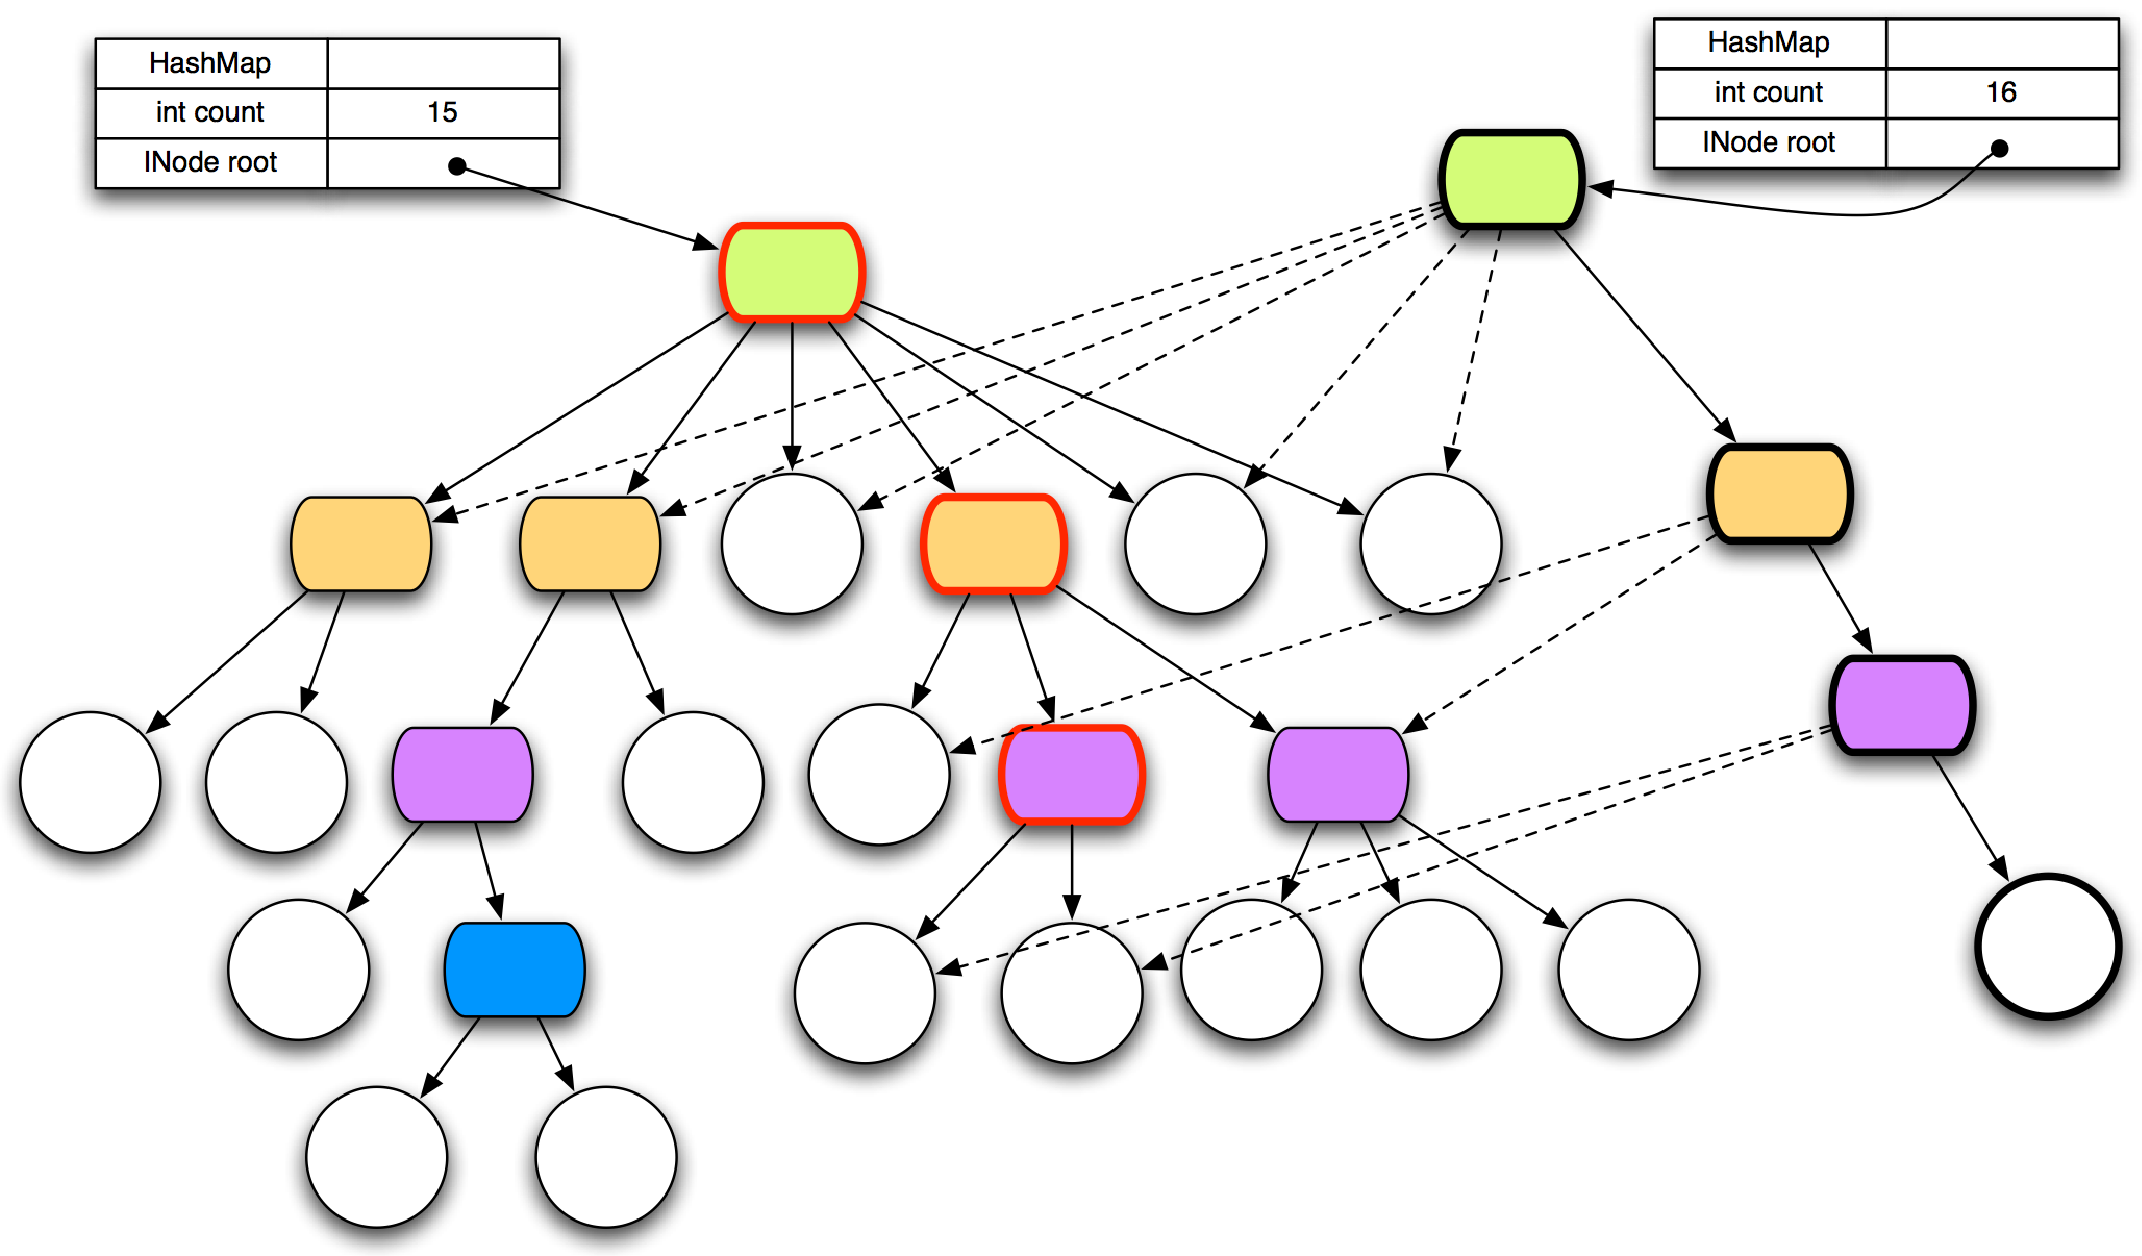
\includegraphics[scale=0.42]{figures/diagrams/persistent-data-structure}
				
				\caption{Representation of how data structures are ``changed'' in Clojure (Source:  \cite{clj-persistent})}
				\label{fig:persistent-data-structure}
			\end{figure}
			
			In \vref{fig:persistent-data-structure}, we see what happens when a persistent data structure is ``changed'' in Clojure.  The root of the left tree is the data structure before, and the root of the right tree is the data structure after.  Note how the changed map retains pointers to all but the updated value; the newly created value is pointed to instead of the previous one.
		
		\subsubsection{Concurrency}
			Clojure supports four systems for concurrency:  \gls{stm}, agents, atoms, and dynamic vars.  The differences between these systems -- including whether or not they are synchronous, coordinated, and what scope they encompass -- are summarized in \vref{tbl:concurrency-system-comparison}.
			
			\begin{table}
				\centering
				
				\begin{tabular}{llll}
					\toprule
					System Name & Synchronous & Coordinated & Scope \\
					\midrule
					\gls{stm} & Yes & Yes & Application \\
					Agents & No & No & Application \\
					Atoms & Yes & No & Application \\
					Dynamic Vars & Not Applicable & Not Applicable & Thread \\
					\bottomrule
				\end{tabular}
				
				\caption{Comparison between Clojure's four systems for concurrency}
				\label{tbl:concurrency-system-comparison}
			\end{table}
			
			In this context, synchronous refers to the fact that each operation waits for the proceeding operation to complete before continuing.  When a system is coordinated, operations occur in a transaction.  If one operation fails, the entire transaction fails and is rolled back.  This results in additional overhead, but is considered safer as the system shall not be left in an inconsistent state as a result of a failed transaction.
			
			\todo{More concurrency}
			
		\subsubsection{Interoperability With the \gls{jvm}}
			\todo{Compare to other functional languages with decent library support}
			Traditionally, functional programming languages have been undesirable for numerous reasons:  compatibility, libraries, portability, availability, packagability, and tools \cite{no-fp-98}.  Clojure attempts to avoid many of these reasons by running on the \gls{jvm}.  The \gls{jvm} allows Clojure to both call and be called by Java and other languages.  It includes syntactic sugar -- features of a language added in order to simplify the language from a human perspective -- to transparently call Java code, as well as make itself available to Java.  This avoids the above issues.
			
			The syntactic sugar provided by Clojure allows for the accessing of object members, the creation of objects, the calling of methods on an instance or class, etc.  Clojure also includes shortcuts to perform multiple operations on the same object.  The syntax is given in \vref{tbl:jvm-interop-syntax}.
			
			\begin{table}
				\centering
				
				\begin{tabular}{lll}
					\toprule
					Operation & Form & Example \\
					\midrule
					Member Access & \texttt{(.<member> <obj> [args])} & \texttt{(.toString 5)} \\
					 & \texttt{(. <obj> <member> [args])} & \texttt{(. 5 toString)} \\
					 & \texttt{(<class>/<member> [args])} & \texttt{(Integer/parseInt ``5'')} \\
					Object Instantiation & \texttt{(<class>. [args])} & \texttt{(Integer. 5)} \\
					 & \texttt{(new <class> [args])} & \texttt{(new Integer 5)} \\
					Multiple Operations & \texttt{(doto <obj> [forms])} & \texttt{(doto (Vector.) (.add 1))} \\
					\bottomrule
				\end{tabular}
				
				\caption{\gls{jvm} interoperability}
				\label{tbl:jvm-interop-syntax}
			\end{table}
			
			We utilize Clojure's \gls{jvm} interoperability to make use of Apache Lucene and \gls{jdbc}.
			
			\begin{figure}
				\begin{singlespaced}
					\begin{pygments}{clj}
(defn ^Directory idx-path
  [path]
  (SimpleFSDirectory. (File. path)))
					\end{pygments}
				\end{singlespaced}
				
				\caption{Clojure code that, given a path, returns a \texttt{Directory} object}
			\end{figure}